\documentclass{article}
\usepackage[utf8]{inputenc}
\usepackage[total={7in, 10in}]{geometry}

\title{AP Chem Determination of $K_{eq}$ Through Spectroscopy Lab}
\author{Theo Urban with Will Bakos and Mikail Jaffer}
\date{Febuary 23 2021}
\usepackage{tabularx}
\usepackage{graphicx}
\usepackage{float} 
\usepackage{pgfplots}
\pgfplotsset{compat=1.17}

\graphicspath{ {./} }

\begin{document}

\maketitle

\section{Purpose}
    The Purpose of this lab is to determine the $K_{eq}$ for the reaction $Fe^{+3}_{aq} + SCN^-_{aq} \rightleftharpoons FeSCN^{+2}_{aq}$ by determining the concentrations of the reactants and products at equilibrium by comparing absorption levels of the resulting solution to a standard curve with known concentrations of reactant.
\section{Data}
\subsection{Standard Curve Data}
\begin{table}[h!]
\centering
    \begin{tabular}{c|c|c|c|c}
        Sample & $[Fe^{+3}]_{initial}$ & $[SCN^-]_{initial}$ & $[FeSCN^{+2}]_{eq}$ & Absorbance \\
        1 & .16M & $4.0\times10^{-5}M$ & $4.0\times10^{-5}M$ & .131 \\
        2 & .14M & $6.0\times10^{-5}M$ & $6.0\times10^{-5}M$ & .197 \\
        3 & .12M & $8.0\times10^{-5}M$ & $8.0\times10^{-5}M$ & .269 \\
        4 & .10M & $1.0\times10^{-4}M$ & $1.0\times10^{-4}M$ & .321 \\
        5 & .080M & $1.2\times10^{-4}M$ & $1.2\times10^{-4}M$ & .417
    
    \end{tabular}
\end{table}
\centering
\textbf{Figure 1}: Reference/Standard Curve - In this set of data, the standard curve is formed by observing the absorbance of a series of reactions where the Iron ion is in large excess, effectively converting all of the Thiocyanate ions into $FeSCN^{+2}$.
$\ $ 

\begin{table}[h!]
    \centering
    \begin{tabular}{c|c|c|c}
        Sample & $[Fe^{+3}]_{initial}$ & $[SCN^-]_{initial}$ & Absorbance \\
        6 & $1.0\times10^{-3}$ & $2.0\times10^{-4}M$ & .089 \\
        7 & $1.0\times10^{-3}$ & $4.0\times10^{-4}M$ & .157 \\
        8 & $1.0\times10^{-3}$ & $6.0\times10^{-4}M$ & .245 \\
        9 & $1.0\times10^{-3}$ & $8.0\times10^{-4}M$ & .327 \\
        10 & $1.0\times10^{-3}$ & $1.0\times10^{-3}M$ & .407 
    \end{tabular}
\end{table}

\centering
\textbf{Figure 2}: Test Solutions - These are the test solutions that were used to determine the $K_{eq}$ for the reaction. They will not react to completion as they have similar enough concentrations of reactants and products.
$\ $
\newpage 
\subsection{Equilibrium Constant Data}
\begin{table}[h!]
    \centering
        \begin{tabular}{c|c|c|c|c}
            Sample & $[FeSCN^{+2}]_{eq}$ & $[Fe^{+3}]_{eq}$ & $[SCN^-_{aq}]$ & $K_{eq}$ \\
            6 & $2.6\times 10^{-5}$ & $9.7\times 10^{-4}$ & $1.7\times10^{-4}$ & 150 \\
            7 & $4.8\times 10^{-5}$ & $9.5\times 10^{-4}$ & $3.5\times10^{-4}$ & 140 \\
            8 & $7.4\times 10^{-5}$ & $9.3\times 10^{-4}$ & $5.3\times10^{-4}$ & 150 \\
            9 & $9.7\times 10^{-4}$ & $9.0\times 10^{-4}$ & $7.0\times10^{-4}$ & 150 \\
            10 & $1.2\times 10^{-4}$ & $8.8\times 10^{-4}$ & $8.8\times 10^{-4}$ & 150\\
            & & &Average&150
        \end{tabular}
    \end{table}

\centering

\textbf{Figure 3}: Results Table(calculated) - $K_{eq}$ is calculated by comparing the absorbance of the reaction to the reference curve using the regression equation.
$\ $

\resizebox{450pt}{!}{%
    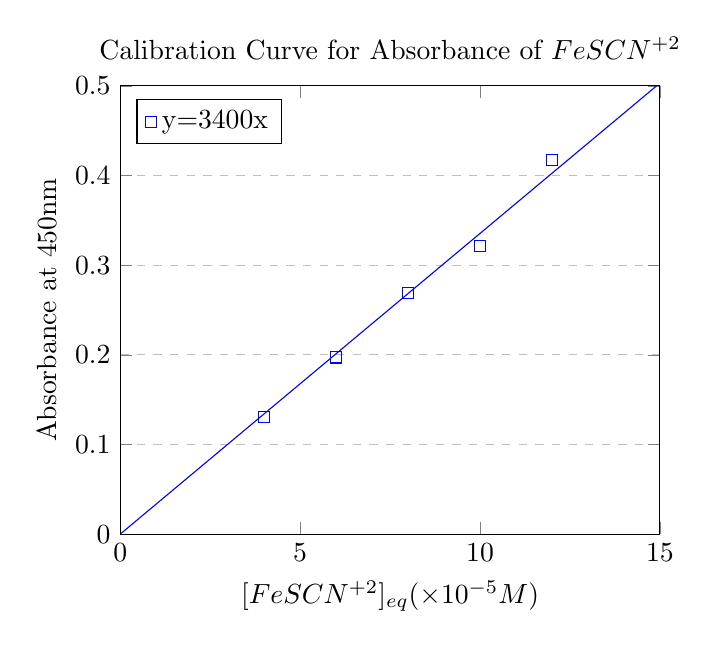
\begin{tikzpicture}
    \begin{axis}[
        title={Calibration Curve for Absorbance of $FeSCN^{+2}$},
        xlabel={$[FeSCN^{+2}]_{eq}(\times 10^{-5}M)$},
        ylabel={Absorbance at 450nm},
        ymin=0, ymax=.5,
        xmin=0, xmax=15,
        xtick={0,5,10,15},
        ytick={0, .1, .2, .3, .4, .5},
        legend pos=north west,
        ymajorgrids=true,
        grid style=dashed,
    ]

    \addplot[
        only marks,
        color=blue,
        mark=square,
        ]
        coordinates {
            (4,.131)
            (6,.197)
            (8,.269)
            (10,.321)
            (12,.417)
        };
        \legend{y=3400x}
    \addplot[thin, draw = blue, mark = none, domain={0:15}] {.0335333*x};

    \end{axis}
    \end{tikzpicture}
}
$\ $ 

\textbf{Figure 4:} Graph of the standard curve points (Complex concentration, absorbance) with the regression line. This allows us to determine an unknown concentration of the ion complex given the absorbance.

\newpage
\section{Calculations}
\subsection{$[FeSCN^{+2}]_{eq}$}
Example from Sample 6: 
$$y=3400x$$
$$.089=3400*[FeSCN^{+2}]_{eq}$$
$$[FeSCN^{+2}]_{eq}=.089/3400 = 2.9\times10^{-5}$$
\subsection{$[Fe^{+3}]_{eq}$}
Example from Sample 6:
$$[{Fe^{+3}_{aq}}]_{eq} = [{Fe^{+3}_{aq}}]_{initial} - [{FeSCN^{+2}_{aq}}]_{eq}$$
$$[{Fe^{+3}_{aq}}]_{eq} = 1.0\times10^{-3} - 2.6\times10^{-5} = 9.7\times10^{-4}$$
\subsection{$[SCN^-_{aq}]$}
Example from Sample 6:
$$[{SCN^{-}_{aq}}]_{eq} = [{SCN^-_{aq}}]_{initial} - [{FeSCN^{+2}_{aq}}]_{eq}$$
$$[{Fe^{+3}_{aq}}]_{eq} = 2.0\times10^{-4} - 2.6\times10^{-5} = 1.7\times10^{-4}$$
\subsection{$K_{eq}$}
Example from Sample 6:
$$K_{eq} = \frac{[FeSCN^{+2}]_{eq}}{[Fe^{+3}]_{eq}[SCN^-]_{eq}}$$
$$K_{eq} = \frac{[2.6\times10^{-5}]}{[9.7\times10^{-4}][1.7\times 10^{-4}]} = 150$$
\subsection{$K_{eq} Averaging$}
$$K_{eq(avg)} = \frac{trial\ 6 K_{eq}+...+trial\ 10 K_{eq}}{5}$$
$$K_{eq(avg)} = \frac{150+140+150+150+150}{5} = 150$$

\newpage
\section{Discussion}
\subsection{Caluclation Approach}

$K_{eq}$ is calculated by comparing the absorbance of the reaction to the reference curve using the regression equation.  The regression equation is calculated by comparing the concentration of $Fe^{+3}_{aq} + SCN^-_{aq} \rightleftharpoons FeSCN^{+2}_{aq}$ with a high concentration of $Fe^{+3}_{aq}$(meaning the reaction goes almost to completion as when the reverse reaction happens, the forward happens again very quickly) after Fe to the absorbance of the reaction at 450nm.  The regression equation is then used to calculate the $K_{eq}$ for the reaction when the equilibrium concentration of $FeSCN^{+2}$ is unknown. We can then calculate the $K_{eq}$ for the reaction using the equation $$K_{eq} = \frac{[FeSCN^{+2}]_{eq}}{[Fe^{+3}]_{eq}[SCN^-]_{eq}}$$ To find the concentrations of Iron and Thiocyanate at equilibrium, we can use the following equations due to the law of conservation of mass.
$$[{Fe^{+3}_{aq}}]_{eq} = [{Fe^{+3}_{aq}}]_{initial} - [{FeSCN^{+2}_{aq}}]_{eq}$$
$$[{SCN^{-}_{aq}}]_{eq} = [{SCN^{-}_{aq}}]_{initial} - [{FeSCN^{+2}_{aq}}]_{eq}$$

\subsection{Error}

The main source of human error in this lab lies in the creation of the correct concentrations of reactants in the reactions.  To mitigate this, 10ml serological pipets were.  The wheel to control volume gave more precise control over the amount of reactants used than other methods, but these pipets were also frequently leaky and at first hard to use correctly, perhaps leading to some error.  

Another possible source of error is in the spectrophotometry process, where it is possible that imperfections in the cuvette either during the blanking process or in testing solution absorbance like fingerprints could make the absorbance readings too high, in turn making the concentration of the complex too high and ultimately making the $K_{eq}$ be higher than reality because it would lead to even lower calculated concentrations of Iron and Thiocyanate at equilibrium(which are in the denominator of the $K_{eq}$ equation). 

A final source of error is in the assumption that all of the Thiocyanate in the reactions to form the standard curve does actually react into the ion complex.  While this is mostly true and the discrepancies from it are likely negligible, it could contribute to the slope of the standard curve line being too high and thus causing lower values for the concentration of the ion at equilibrium.  This would in turn result in lower values of $K_{eq}$ because the numerator would decrease and the denominator would increase as well.
\end{document}

